\subsubsection{Breve descripción de cloud computing y web services}

''Procesamiento en la nube'' o \emph{cloud computing} es una expresión que hace referencia a la posibilidad de 
realizar gran variedad de cómputos utilizando un conjunto de muchas máquinas conectadas entre sí 
(cluster). El término ''nube'' intenta describir la abstracción del cluster en sí mismo como componente físico.

El usuario (donde usuario puede ser un individuo, una empresa o cualquier otro tipo de
organización) 
es consciente de que los cómputos que él necesita realizar se efectúan en algún sitio con los componentes
de hardware necesarios pero no requiere saber dónde. El procesamiento es realizado por alguna de las computadoras,
de alguno de los clusters de la nube.

Este sistema intenta maximizar la efectividad de los cómputos de todos los usuarios 
y disminuír el precio al compartir los recursos.
Los mismos no solo son compartidos por distintos usuarios sino que también la cantidad de recursos asignados
para un mismo usuario varía según distintos factores (como por ejemplo la demanda de procesamiento en un
determinado período de tiempo), por lo que el sistema se vuelve muy flexible y permite que las aplicaciones
que utilizan la nube escalen a medida que crezcan en tama\~no (volumen de datos
o de cómputo, cantidad de usuarios, etc).

Paralelamente al desarrollo de ''cloud computing'', empresas como Amazon, Google, dotCloud, Red Hat, etc. comenzaron
a ofrecer lo que conocemos como ''web servicies'': ofrecer al usuario la posibilidad de utilizar el poder de cómputo
de sus computadoras y clusters a cambio de una determinada suma de dinero. Si bien el servicio es pago, incluye
todas las ventajas de la computación en la nube. El servicio es muy flexible y logra que los clientes paguen
únicamente por los recursos que utilizan (y no más que eso). Para cumplir con estos objetivos utilizan el montaje de
máquinas virtuales sobre computadoras físicas. De esta manera son las máquinas virtuales las que son ofrecidas
a los clientes. Estos últimos pueden pagar por más máquinas o menos dependiendo de la demanda de sus aplicaciones.
Al mismo tiempo es posible pagar por más o menos tiempo para cada una.

~

Ya hemos definido la arquitectura del cluster de MongoDB que necesitábamos para nuestra base de datos. Ahora es
momento de analizar distintas alternativas de web services y elegir la que mejor se adapte a nuestras necesidades.

\subsubsection{Amazon}


Ec2 (''elastic computing cloud'') es una rama muy importante dentro de ''Amazon web servicies'' .
El mismo está basado en AMI's (Amazon Machine Images). Cada machine image puede generar una o miles de instancias,
en donde cada instancia es equivalente a una de las máquinas virtuales mencionadas anteriormente.


Según la documentación
oficial de MongoDB (http://docs.mongodb.org/ecosystem/platforms/amazon-ec2/), mongo es compatible con Amazon Ec2.
En suma, existen 3 AMI's oficiales: 

~

\begin{description}
	\item MongoDB 2.4 with 1000 IOPS - data: 200 GB @ 1000 IOPS, journal: 25 GB @ 250 IOPS, log: 10 GB @ 100 IOPS
	\item MongoDB 2.4 with 2000 IOPS - data: 200 GB @ 2000 IOPS, journal: 25 GB @ 250 IOPS, log: 15 GB @ 150 IOPS
	\item MongoDB 2.4 with 4000 IOPS - data: 400 GB @ 4000 IOPS, journal: 25 GB @ 250 IOPS, log: 20 GB @ 200 IOPS
\end{description}

~

Todas ellas tienen una arquitectura basada en 64-bits, Linux/Unix como sistema operativo, un espacio reservado
para almacenar la información de journal y log de la base de datos. Además cuentan con EBS (''elastic block store''),
que posibilitan el almacenamiento permanente de los datos más allá de la vida de la instancia. 
Las máquinas son muy eficientes en el almacenamiento de datos con una gran cantidad operaciones de entrada y salida
por segundo y permiten aprovechar y explotar todas las funcionalidades de MongoDB, como búsqueda completa por índices
(incluídos compuestos y geoespaciales)

~

Las máquinas que nos ofrecen son del tipo: M3 (propósito general) o High-Memory (optimizadas en el uso de memoria RAM).

~

Recordando la configuración inicial de nuestra arquitectura, requeríamos de 2 query routers, 3 config servers y 2 shards.
Cada shard estaba compuesto a su vez por 3 nodos: uno primario y 2 secundarios. 
Por lo tanto, con esta alternativa deberíamos comenzar con 6 AMI's MongoDB 2.4 with 4000 IOPS de tipo de instancia
High-Memory (para cada uno de los nodos que van a contener los datos). En suma deberíamos agregar 5 ami's de propósito
general para los query routers y config servers: Las instancias del tipo M1 y M3 proveen un balance entre cómputo, 
memoria y recursos de red.

~

Otra posibilidad en vez de utilizar las máquinas proupestas por el manual para los nodos de los shrads
consiste en utilizar instancias
optimizadas para almacenamiento: I2 y HI1. (http://aws.amazon.com/ec2/instance-types/). Las mismas están optimizadas
para obtener una gran densidad de almacenamiento con bajo costo, y una gran performance en operaciones de I/0.
Los discos son SSD.
Estas instancias funcionan muy bien con bases de datos noSQL, como mongoDB.

Se incluyen a continuación algunos detalles y precios de instancias I2, m2(memory optimized)
y m3 (general purplse) disponibles:

\begin{center}
    \small{
    \begin{tabular}{| l | l | l | l | l | l | l | l | l |}
    \hline
    Instance family & Type & Arch & vCPU & ECU & Memory(GB) & Storage (GB) & EBS-opt & Network perf\\ \hline
    general purpose & m3.xlarge & 64-bits & 4 & 13 & 15 & 2x40 SSD & yes & Moderate \\ \hline
    memory optimized & m2.xlarge & 64-bits & 2 & 6.5 & 17.1 & 1x420 & no & Moderate \\ \hline 
    storage optimized & i2.xlarge & 64-bits & 4 & 14 & 30.5 & 1x800 SSD & yes & Moderate  \\ \hline
    \end{tabular}
    }
\end{center}

~

La elección de Amazon como proveedor de web-services nos posibilita la 
la incorporación de S3, en el caso de que queramos combinar mongoDB con otro tipo de tecnologías
: Simple storage service. Una interfaz
utilizada para almacenar y envíar datos a cualquier lugar de la web. Los procedimientos se realizan de forma segura,
confiable, rápida y con precios accesibles de forma tal que nuestra aplicación pueda escalar a medida que el volumen
de transferencias sea cada vez mayor. (http://aws.amazon.com/s3/)

~

Finalmente podemos utilizar Ec2 Auto-Scaling con las condiciones que habíamos definido anteriormente (duplicar
la cantidad de AMI's en los casos en donde los datos superen los $\frac{3}{4}$ o disminuyan a menos de $\frac{1}{4}$,
o cuando sea necesario aumentar o disminuir la cantidad de query routers). De esta manera podemos aprovechar la 
flexibilidad del servicio pagando únicamente por los recursos que efectivamente estamos consumiendo:
http://aws.amazon.com/autoscaling/.


\subsubsection{Google compute engine}

De forma similar a Amazon, y compartiendo las mismas ideas y beneficios, Google es otra de las alternativas para 
montar nuestro cluster de mongoDB a través de ''Google compute engine''. Esta empresa nos ofrece la misma 
infraestructura que utiliza para realizar billones de búsquedas en milisegundos, administrar millones de cuentas
de gmail, etc. 

A su vez permite combinar sus servicios de cómputo, almacenamiento y funcionalidades (a través de Google API's).

Las opciones que nos ofrece Google compute engine son similares a las Ec2 de Amazon: Máquinas de propósito general,
optimizadas para procesamiento y optimizadas para el manejo de la memoria. Estas últimas son las que nos interesan
como plataforma en donde almacenar los datos de nuestra aplicación.

Dentro de las características especiales que ofrece el servicio, una de las más importantes es la velocidad y robustez
de las transferencias utilizando la red global de google. Además brinda un servicio de balanceo para distribuír los 
datos en diversas instancias disminuyendo el tráfico de la red y aumentando la performance de nuestra aplicación.

Finalmente, así como Amazon ofrecía el servicio de S3, google provee \emph{Cloud storage o Cloud Datastore}, en el
caso de que queramos combinar mongoDB con otras tecnologías. 

Si bien ''Google compute engine'' no está incluída como opción en el conjunto de plataformas que soporta mongoDB 
mencionadas en el manual (http://docs.mongodb.org/ecosystem/platforms/), actualmente existe dicho soporte. 
Las capacidades de la infraestructura de GCE hacen que la base de datos pueda funcionar muy satisfactoriamente, 
principalmente por la velocidad de la red que hemos mencionado más arriba:
http://blog.mongolab.com/2013/05/mongolab-now-supports-google-cloud-platform/

\subsubsection{dotCloud}

MongoDB puede correr en las plataformas que ofrece ''dotCloud''. Las mismas soportan \emph{replica sets} y sharding.
La principal ventaja de dotCloud es que permite correr las aplicaciones y mantener la base de datos en un mismo lugar
para optimizar la latencia y confiabilidad.

Por estos motivos, dotCloud aparece como segunda alternativa en la documentación de plataformas de mongo.
(http://docs.mongodb.org/ecosystem/platforms/dotcloud/).

Para inicializar nuestra aplicación podemos olvidar la arquitectura diseñada previamente y dejar que dotCloud realice
las configuraciones de escalabilidad de manera automática. 

Por lo tanto simplemente debemos elegir los servicios que va a requerir la aplicación, incluyendo 
lógicamente entre ellas mongoDB para la elección de la base de datos.

(https://www.dotcloud.com/howitworks.html)


\subsubsection{Escalabilidad lineal}

La utilización de \emph{Haas} como medio para albergar nuestra base de datos es una muy buena opción. Además de los motivos
anteriormente mencionados, uno muy importante es que la inversión inicial es muy baja. No es necesario pagar por adelantado.
Simplemente se paga por los recursos  utilizados. En cuanto haya recursos pedidos que no están siendo utilizados, fácilmente
podemos dejar de contratarlos y (por lo tanto) dejar de pagarlos.

Suponiendo que el primer a\~no tengamos un gasto de $x$ por haber pedido recursos (como por ejemplo, las distintas AMI's de
Ec2 de Amazon), se espera que el siguiente tengamos un gasto de $cx$, donde $c$ es una constante. Lo mismo para los a\~nos
siguientes. Por lo tanto, la empresa probablemente pueda afrontar los gastos a\~no tras a\~no, considerando que 
la inversión durante el primer a\~no no es tan alta, y que los ingresos que genera la aplicaci\'on son suficientes (no
necesariamente demasiado elevados).

Por lo tanto la solución propuesta mediante \emph{Haas} escala a nivel económico.

\subsubsection{Migración a Hardware propio}

Si en un futuro la empresa decidiera cambiar la implementación \emph{Haas} por una de hardware propio podrían surgir 
grandes riesgos especialmente a nivel económico:

En primer lugar la inversión inicial que habría que hacer sería muy grande, especialmente si la aplicación cuenta para
esa altura con muchos clientes y una base de datos considerablemente grande.

En segundo lugar debería destinarse una porción de los recursos económicos a la creación de un departamento de
mantenimiento del hardware enfocado a bases de datos de gran tama\~no. (Dentro del mismo, deberían tratarse temas
como por ejemplo backup de datos y seguridad, como los que aprendimos en la segunda mitad de la materia. Entre
ellos, distintos niveles de RAID para proteger los datos).

En suma, la empresa no contaría con la suficiente flexibilidad como para afrontar las subas y bajas de la demanda:
Se pierde el concepto de escalar hacia abajo porque deja de ser viable ''tirar o vender'' el hardware sobrante.
Al mismo tiempo, escalar hacia arriba pasa a ser algo riesgoso, ya que cada vez que se quiera ampliar la capacidad
de la base no va a saberse con certeza si la compra está justificada o no.

Una solución parcial sería brindar un web-service propio con el hardware propio, aunque eso no es algo para nada fácil.
Por un lado debería haber empleados que se dediquen a brindar ese servicio, y por el otro la empresa debería competir
con otras como Amazon o Google.

En resumen, la migración de \emph{Haas} hacia hardware propio no parece algo demasiado seguro .


\subsubsection{Hecho real: Reddit sobre Amazon Ec2}

Reddit es una página de internet en donde los usuarios postean, comentan y votan
ideas, hechos y acontecimientos de interés general. Actualmente el sitio corre enteramente sobre AWS Ec2, y escala
exitosamente mes tras mes, lo que le posibilita poder manejar hasta 4 billones de visitas a su página por mes.
Según Keith Mitchell (programador del sitio), en un video que podemos ver en: 
http://aws.amazon.com/solutions/case-studies/reddit/ (link desde la página oficial de aws), explica que 
la empresa migró de tener sus propios servidores físicos a contratar los servicios de Amazon obteniendo resultados
asombrosos. Anteriormente disponían de 5 equipos completos de mantenimiento de hardware (hecho que resultaba
costoso). La empresa cuenta actualmente con menos de 20 empleados, y este hecho no les impide manejar el volumen de
datos que maneja. Debido al encapsulamiento que provee el uso de web-services,
pueden enfocarse en cuestiones como el código de la aplicación en sí mismo, o aspectos publicitarios.

~

\begin{figure}[!h]
    \begin{center}
          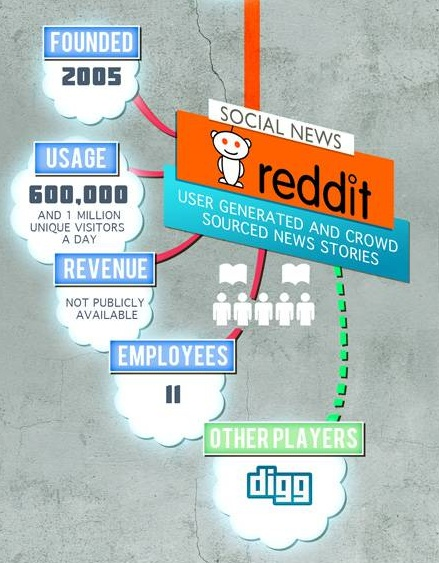
\includegraphics[scale=0.4]{imagenes/im_2.jpg}
          \caption{Esquema gráfico: datos reales de Reddit}
          \label{fig:contra1}
    \end{center}
\end{figure}
\FloatBarrier
